\chapter{Formal analysis using Alloy}

Here we present the specification of the system described above using Alloy. The goal of this specification is to model a system that ensures the integrity and correctness of constraints related to internship applications, student eligibility, and system behaviors.

The specification is structured around a set of signatures: users, students, companies, internships, and universities. Each entity is defined with its attributes and relationships. For instance, students are modeled as users with additional attributes like their applied internships, current internship work, CV, and associated university.

Facts are also introduced to define constraints. These includes that no two users can share the same email, a student cannot apply for an internship without a CV, and only one student can work in a given internship at a time. Additional constraints verify that students can only be rejected from internships they have previously applied to, and historical rules ensure that a CV always belongs to a single student throughout the system's lifecycle.

We used predicates to define dynamic operations such as students applying for internships, starting work, or being rejected. A global "eventsFact" encapsulates the control flow of these operations to maintain consistency within the system.

Finally, a world predicate establishes initial conditions for the system, such as ensuring there are more than two students, companies, and internships in the environment

\vspace{2cm}
\lstinputlisting[language=alloy]{Alloy/RASD_ALLOY.als}

\subsubsection*{Examples}

In this scenario, there are two companies: one is offering three internships, while the other is offering a single internship. We also have three students studying at the same university.

\begin{figure} [H]
    \centering
    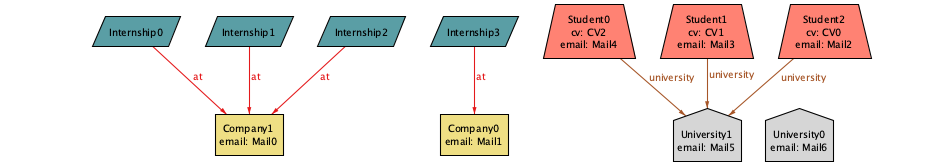
\includegraphics[width=1\linewidth]{Alloy/State.png}
    \caption{State 0}
\end{figure}

At the first step Student0 applies for Internship0.

\begin{figure} [H]
    \centering
    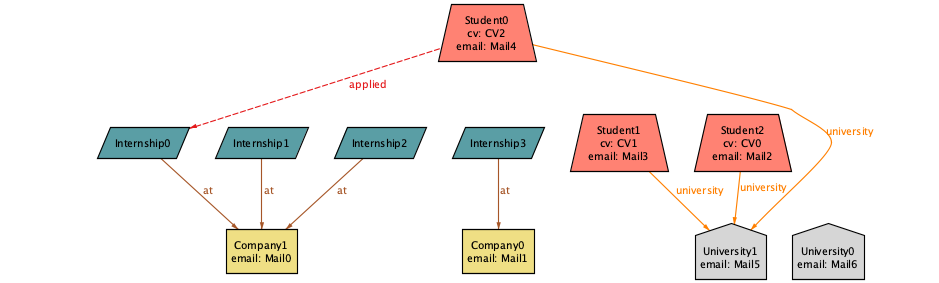
\includegraphics[width=1\linewidth]{Alloy/State1.png}
    \caption{State 1}
\end{figure}

At the second step, Student2 applies for Internship1 but gets rejected.

\begin{figure} [H]
    \centering
    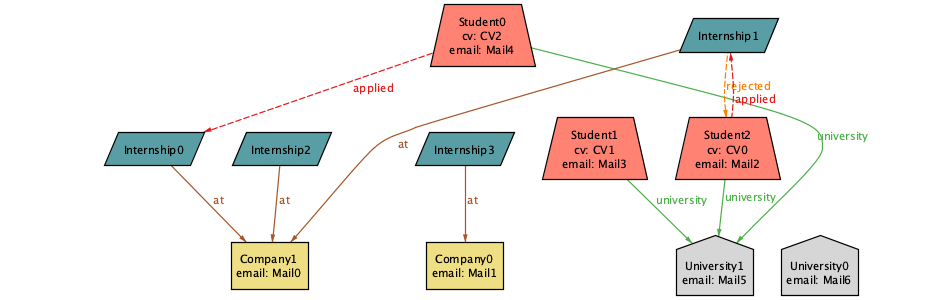
\includegraphics[width=1\linewidth]{Alloy/State2.png}
    \caption{State 2}
\end{figure}

At the third step, Student0 applies for Internship3 while Student2 applies for Intership0

\begin{figure} [H]
    \centering
    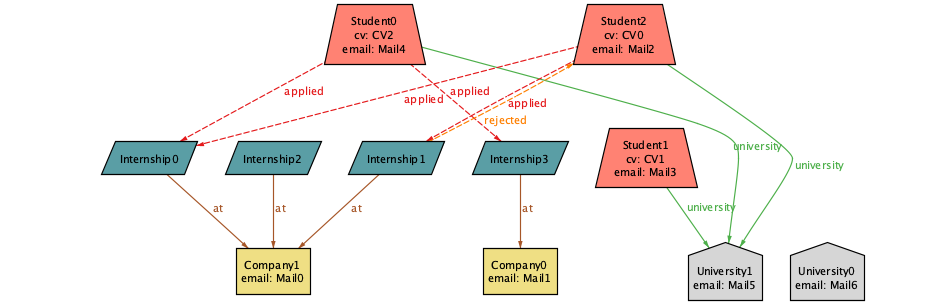
\includegraphics[width=1\linewidth]{Alloy/State3.png}
    \caption{State 3}
\end{figure}

At the fourth step, Student0 gets accepted and starts working on Internship3. 

\begin{figure} [H]
    \centering
    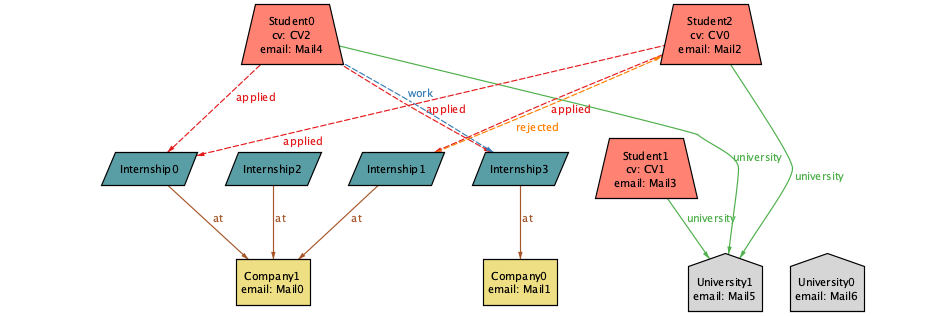
\includegraphics[width=1\linewidth]{Alloy/State4.png}
    \caption{State 4}
\end{figure}

At the fifth step, Student2's application to Internship0 gets rejected.

\begin{figure} [H]
    \centering
    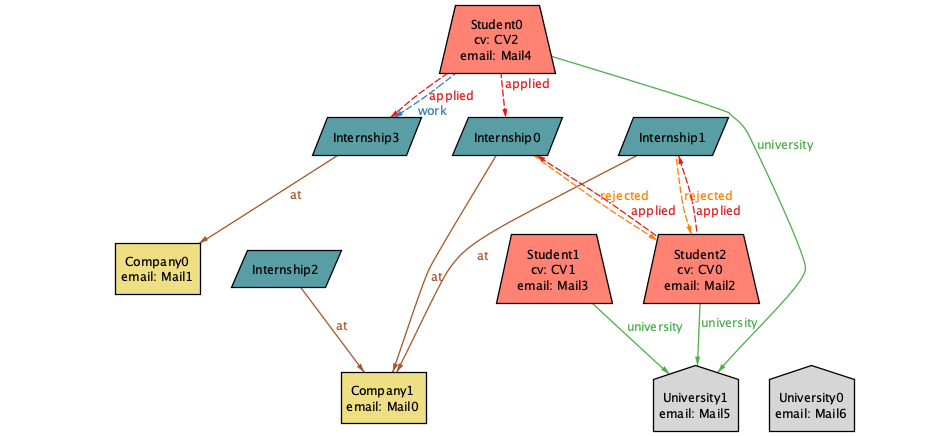
\includegraphics[width=1\linewidth]{Alloy/State5.png}
    \caption{State 5}
\end{figure}

At the sixth step, Student1 applies for Internship0

\begin{figure} [H]
    \centering
    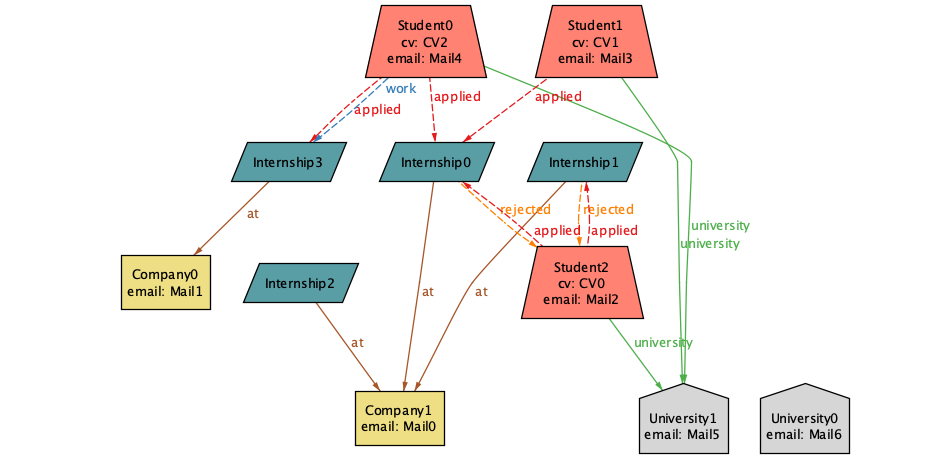
\includegraphics[width=1\linewidth]{Alloy/State6.png}
    \caption{State 6}
\end{figure}